\documentclass[handout]{beamer}
\usepackage{multicol}
\usepackage{xy}
\everymath{\displaystyle}
\mode<presentation>
{\usetheme{Warsaw}\setbeamercovered{dynamic}}
\usecolortheme{crane}
\usepackage{beamerfoils}
\pgfdeclareimage[height=1in]{university-logo}{ISULogo}
\logo{\pgfuseimage{university-logo}}
\setbeamertemplate{navigation symbols}{}
\title[Blackjack]{Blackjack}
\author{Dr Marcus Bishop}
\subject{Math 104}
\beamerdefaultoverlayspecification{<+->}
\theoremstyle{definition}
\newtheorem{remark}{Remark}
\newtheorem{impact}{Impact}
\newtheorem{situation}{Situation}
\newtheorem{question}{Question}
\usepackage{arev}
\usepackage{tensor}
\newcommand\npr[2]{\tensor[_{#1}]P{_{#2}}}
\newcommand\ncr[2]{\tensor[_{#1}]C{_{#2}}}
\usepackage{cancel}
\newcommand{\hs}{\alert{\varheart}}
\newcommand{\ds}{\alert{\vardiamond}}
\newcommand{\s}{\spadesuit}
\newcommand{\cs}{\clubsuit}
\begin{document}
\begin{frame}\titlepage\end{frame}
\LogoOff

\begin{frame}{Blackjack}
\begin{itemize}
\item We consider casino version
\item Also exists friendly version
\item In casino version player play against dealer, not against one another
\item Each player makes bet
\item Dealer deals each player two face-up cards
\item She also deals herself one face-up, one face-down
\item $J,K,Q$ worth $10$~points
\item $A$ worth either $1$ or $11$~points, whichever convenient
\item Remaining cards worth value shown on card
\end{itemize}
\end{frame}

\begin{frame}
\begin{itemize}
\item If player's sum exactly $21$ (a \alert{blackjack}) player wins
$\frac{3}{2}$ amount bet
\item Players can request further cards, as many as desired
\item Accomplished by saying \alert{hit me}
\item Sum of player's cards should be as close to $21$ as possible
without exceeding $21$
\item If sum exceeds $21$ player loses bet (a \alert{bust})
\item When remaining players (if any) satisfied with their sums
(they \alert{stand}) dealer reveals her
face-down card
\item If she has blackjack, remaining players lose bets
\item \dots unless they also have blackjack
\item No money exchanged if player and dealer both have blackjack
\end{itemize}
\end{frame}

\begin{frame}
\begin{itemize}
\item Dealer hits herself as needed
\item She \alert{must} hit herself if her sum $\le 16$
\item However, she must stop hitting herself when her sum $\ge 17$
\item If her sum $>21$ (she \alert{busts}), player wins amount bet
\item Suppose her sum $\le 21$
\item If her sum closer to $21$ than player's sum,
player loses bet
\item If player's sum closer to $21$ than dealer's sum,
player wins amount bet
\item \dots unless player's sum $21$
\item Then player wins $\frac{3}{2}$ amount bet
\item If dealer's sum equals player's sum, no money exchanged
\end{itemize}
\end{frame}

\begin{frame}{Why blackjack favors casino}
\begin{itemize}
\item Game sounds perfectly symmetric: dealer as likely
as player to arrive at sum closest to $21$
\item Why does game favor casino?
\item If player busts, player loses automatically
\item Dealer doesn't even need to hit herself if player busts
\item If she does hit and busts, player still loses
\end{itemize}
\end{frame}

\begin{frame}{Probability of blackjack}
\begin{itemize}
\item Two cards whose sum $21$ called a \alert{blackjack}
\item If player receives blackjack in first two cards,
he wins unless dealer also has blackjack
\item Calculate probability of receiving blackjack on first two cards
\item Can only happen if one card is $A$ and other
has value $10$
\item So other card must be $10$, $J$, $Q$, or $K$
\item Four choices for $A$
\item $16$~choices for other card
\item So $4\cdot 16=64$ blackjacks possible
\item $\ncr{52}{2}=1326$ two-card hands possible 
\item So $\frac{64}{1326}\approx 0.0483$ the probability of blackjack
\item We'll round answer to $\frac{1}{20}$
\end{itemize}
\end{frame}

\begin{frame}{Remarks}
\begin{itemize}
\item All our blackjack calculations only approximate
\item One issue: dealer often uses several decks of cards, rather than one
\item So $\frac{1}{52}$ the
approximate probability of receiving any particular card
\item \dots even though card might already appear on table
\item $\frac{1}{13}$ the probability of receiving card
of any particular rank
\item Casino's use of several decks probably intended to foil
intentions of \alert{card counters} (discussed later)
\item Blackjack can be played virtually at
\href{http://wizardofodds.com/play/blackjack}{\color{blue}\tt wizardofodds}
\end{itemize}
\end{frame}

\begin{frame}{Probability of winning with blackjack}
\begin{itemize}
\item If player receives blackjack
%(with probability $\approx\frac{1}{20}$
what is probability he wins?
\item Player loses only if dealer also has blackjack
\item Dealer has blackjack with probability $\textstyle\frac{1}{20}$
\item So player wins with probability $\textstyle\frac{19}{20}$
\item So $\frac{1}{20}\cdot\frac{19}{20}
\approx\frac{1}{20}$ the probability of getting blackjack and winning
\end{itemize}
\begin{remark}
\begin{itemize}
\item Player receiving blackjack and dealer not receiving blackjack
not independent
\item So strictly speaking 
$\frac{1}{20}\cdot\frac{19}{20}$ incorrect
\item However, suffices for approximate calculation
\end{itemize}
\end{remark}
\end{frame}

\begin{frame}{Probability of busting if hit}
\begin{itemize}
\item Most important question: should player take another card?
\item Want to calculate probability that player busts
if hit
\item Depends on cards player has
\item Will assume several decks being used
\end{itemize}
\begin{example}
\begin{itemize}
\item Suppose player has $J\hs,5\cs$
\item Ranks that \alert{won't} bust player:
$A,2,3,4,5,6$
\item $\frac{6}{13}$ the probability player won't bust if hit
\item So $\frac{7}{13}$ the probability player busts if hit
\end{itemize}
\end{example}
\end{frame}

\begin{frame}{Probability distribution of blackjack}
\begin{itemize}
\item Want to calculate probability player winds up with particular sum
\item To simplify problem, suppose player follows dealer's rule
\item Namely, he hits if his sum $\le 16$, stands if $\ge 17$
\item So possible outcomes $17,18,19,20,21$ or blackjack or bust
\item Have already calculated probability of blackjack
\item Remaining outcomes too difficult to calculate,
since each outcome can happen in many ways
\end{itemize}
\end{frame}

\begin{frame}
\begin{itemize}
\item List shows all ways to get sum of $17$
\item List has $267$ entries
\item \alert{T} denotes $10$, $J$, $Q$, or $K$
\item So each entry containing \alert{T}
represents $4$ outcomes
\end{itemize}
\tiny
2222AAAAAAAAA 22222AAAAAAA 222222AAAAA 2222222AAA 22222222A 322AAAAAAAAAA 
3222AAAAAAAA 32222AAAAAA 322222AAAA 3222222AA 32222222 332AAAAAAAAA 
3322AAAAAAA 33222AAAAA 332222AAA 3322222A 333AAAAAAAA 3332AAAAAA 
33322AAAA 333222AA 3332222 3333AAAAA 33332AAA 333322A 
33333AA 333332 422AAAAAAAAA 4222AAAAAAA 42222AAAAA 422222AAA 
4222222A 43AAAAAAAAAA 432AAAAAAAA 4322AAAAAA 43222AAAA 432222AA 
4322222 433AAAAAAA 4332AAAAA 43322AAA 433222A 4333AAAA 
43332AA 433322 43333A 44AAAAAAAAA 442AAAAAAA 4422AAAAA 
44222AAA 442222A 443AAAAAA 4432AAAA 44322AA 443222 
4433AAA 44332A 44333 444AAAAA 4442AAA 44422A 
4443AA 44432 4444A 52AAAAAAAAAA 522AAAAAAAA 5222AAAAAA 
52222AAAA 522222AA 5222222 53AAAAAAAAA 532AAAAAAA 5322AAAAA 
53222AAA 532222A 533AAAAAA 5332AAAA 53322AA 533222 
5333AAA 53332A 53333 54AAAAAAAA 542AAAAAA 5422AAAA 
54222AA 542222 543AAAAA 5432AAA 54322A 5433AA 
54332 544AAAA 5442AA 54422 5443A 5444 
55AAAAAAA 552AAAAA 5522AAA 55222A 553AAAA 5532AA 
55322 5533A 554AAA 5542A 5543 555AA 
5552 62AAAAAAAAA 622AAAAAAA 6222AAAAA 62222AAA 622222A 
63AAAAAAAA 632AAAAAA 6322AAAA 63222AA 632222 633AAAAA 
6332AAA 63322A 6333AA 63332 64AAAAAAA 642AAAAA 
6422AAA 64222A 643AAAA 6432AA 64322 6433A 
644AAA 6442A 6443 65AAAAAA 652AAAA 6522AA 
65222 653AAA 6532A 6533 654AA 6542 
655A 66AAAAA 662AAA 6622A 663AA 6632 
664A 665 7AAAAAAAAAA 72AAAAAAAA 722AAAAAA 7222AAAA 
72222AA 722222 73AAAAAAA 732AAAAA 7322AAA 73222A 
733AAAA 7332AA 73322 7333A 74AAAAAA 742AAAA 
7422AA 74222 743AAA 7432A 7433 744AA 
7442 75AAAAA 752AAA 7522A 753AA 7532 
754A 755 76AAAA 762AA 7622 763A 
764 77AAA 772A 773 8AAAAAAAAA 82AAAAAAA 
822AAAAA 8222AAA 82222A 83AAAAAA 832AAAA 8322AA 
83222 833AAA 8332A 8333 84AAAAA 842AAA 
8422A 843AA 8432 844A 85AAAA 852AA 
8522 853A 854 86AAA 862A 863 
87AA 872 88A 9AAAAAAAA 92AAAAAA 922AAAA 
9222AA 92222 93AAAAA 932AAA 9322A 933AA 
9332 94AAAA 942AA 9422 943A 944 
95AAA 952A 953 96AA 962 97A 
98 TAAAAAAA T2AAAAA T22AAA T222A T3AAAA 
T32AA T322 T33A T4AAA T42A T43 
T5AA T52 T6A T7 AAAAAAA A2AAAA 
A22AA A222 A3AAA A32A A33 A4AA 
A42 A5A A6

\end{frame}

\begin{frame}
Nevertheless, can use computer to calculate
distribution:\footnote{Source:
\href{http://www.wiley.com/WileyCDA/WileyTitle/productCd-0470624450.html}
{\color{blue}
{\em Probabilities: the Little Numbers that Rule Our Lives},
by Peter Olofsson}}
\[\begin{array}{r|lllllll}
r&17&18&19&20&21&\text{Blackjack}&\text{Bust}\\\hline
P\left(r\right)&0.15&0.15&0.14&0.18&0.05&0.05&0.28
\end{array}\]
\begin{example}
\begin{itemize}
\item Suppose you wind up with $17$
\item Calculate probability that you win
\item You lose if dealer has $18,19,20,21$ or blackjack
\item According to table above,
occurs with probability $0.15+0.14+0.18+0.05+0.05=0.57$
\item You tie (or \alert{push})
if dealer has $17$, with probability $0.15$
\item You win if she busts, with probability $0.28$
\end{itemize}
\end{example}
\end{frame}

\begin{frame}{One strategy}
\begin{itemize}
\item One possible strategy from
\href{http://www.wiley.com/WileyCDA/WileyTitle/productCd-0470624450.html}
{\color{blue}Olofsson}:
\begin{itemize}
\item If sum $\le 11$ hit (can't possibly exceed $21$ by hitting)
\item If dealer has $7$ or greater face-up, continue hitting until
sum $\ge 17$
\item If dealer has $2,3,4,5$ or $6$ face-up, continue hitting
until sum $\ge 12$
\item \dots unless sum exactly $12$ and dealer has $2$ or $3$
face-up; then hit
\end{itemize}
\item Strategy comes with no guarantee
\item More complicated strategies exist, often resulting
from computer simulation involving millions of games
\end{itemize}
\end{frame}

\begin{frame}{Card counting}
\begin{itemize}
\item Listen to
\href{http://www.thisamericanlife.org/radio-archives/episode/466/blackjack}
{\color{blue}This American Life} episode on card counting
\item Observe that deck rich in high cards favors player because
\begin{itemize}
\item Dealer must hit until her sum $\ge 17$
\item \dots but higher cards more likely to bust her
\item Also, blackjacks more likely if deck has many higher cards
\item However, she pays you $\frac{3}{2}$ amount bet
if you receive blackjack
\item \dots but she only receives your bet if she receives blackjack
\end{itemize}
\item Conversely deck rich in low cards favors dealer
\end{itemize}
\end{frame}

\begin{frame}
\begin{itemize}
\item But how to know if deck rich in high cards?
\item By keeping track!
\item Hi-lo method:
\begin{itemize}
\item When dealer shuffles, player keeps running tally,
beginning with zero
\item Player adds one every time dealer deals $2,3,4,5,6$
\item Player subtracts one every time dealer deals $10,J,K,Q,A$
\item When tally reaches $+10$, say, player should bet more
\item When tally negative, player should bet less
\end{itemize}
\item Can practice at \href{http://www.random.org/playing-cards}
{\color{blue}\tt random.org}
\item Players began card counting in 1960's with publication
of Edward O. Thorp's 1962 book {\em Beat the Dealer}
\item Casinos responded to card counters by using several decks,
shuffling more often, harassing suspected counters, etc.
\end{itemize}
\end{frame}

\begin{frame}{Monty Hall Problem}
\begin{center}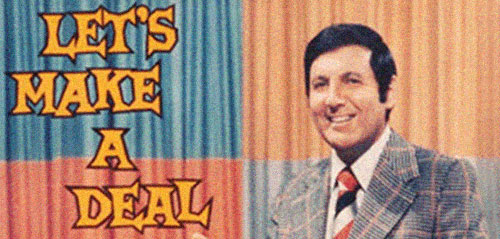
\includegraphics[scale=.5]{LetsMakeDeal}\end{center}
\begin{itemize}
\item \alert{Let's Make a Deal} a TV game show
initiated in 1963
\item Monty Hall the original host
\item Content of game varies, but essentially
consists of contestants choosing among known and unknown prizes
\item Some prizes valuable, other worthless
\end{itemize}
\end{frame}

\begin{frame}
\begin{center}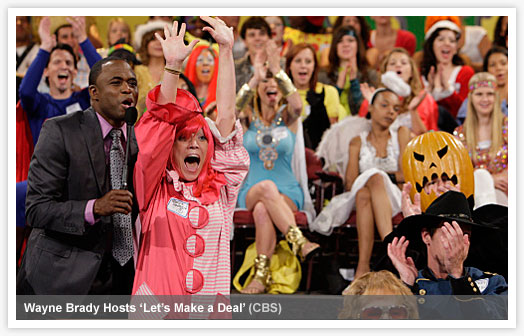
\includegraphics[scale=.5]{WayneBrady}\end{center}
\begin{itemize}
\item Today program runs on CBS daytime TV
\item Debuted in 2009, hosted by Wayne Brady
\item Contestants generally arrive in costume
to increase odds of being selected to play
\end{itemize}
\end{frame}

\begin{frame}
\begin{center}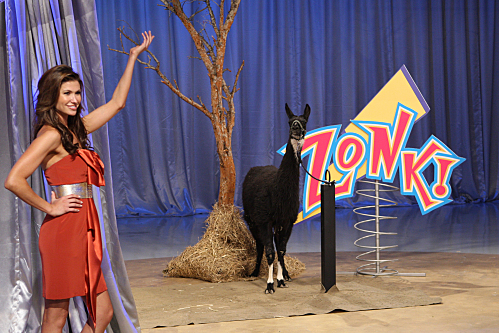
\includegraphics[scale=1.25]{Goat}\end{center}
\begin{itemize}
\item Possibility exists that player wins worthless prize
\item Live goat shown here
\end{itemize}
\end{frame}

\begin{frame}
\begin{center}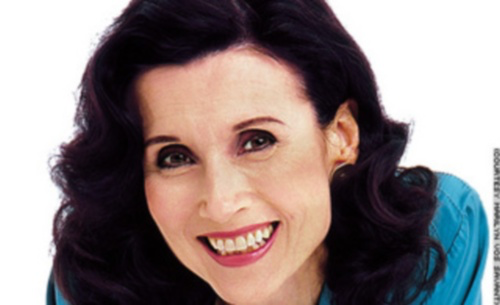
\includegraphics[scale=.5]{VosSavant}\end{center}
\begin{itemize}
\item Marilyn vos Savant writes \alert{Ask Marilyn}
column in \alert{Parade} magazine
\item Parade the most widely read magazine in US
\item Column initiated in 1986, consists of solutions
to readers' puzzles, dilemmas, etc
\item vos Savant the holder of \alert{Guinness Book of World Records}
highest IQ record 1986--1989
\item Link to \alert{Ask Marilyn} featured prominently on
\href{http://parade.com}{\color{blue}Parade webpage}
\end{itemize}
\end{frame}

\begin{frame}
\begin{itemize}
\item Following letter appears in \alert{Ask Marilyn} in 1990:
\item\begin{quotation}
Suppose you're on a game show, and you're given the choice of three
doors: Behind one door is a car; behind the others, goats. You pick
a door, say No. 1, and the host, who knows what's behind the doors,
opens another door, say No. 3, which has a goat. He then says to
you, "Do you want to pick door No. 2?" Is it to your advantage to
switch your choice?
\end{quotation}
\item Can play simulation of reader's scenario
\href{http://math.ucsd.edu/~crypto/Monty/monty.html}
{\color{blue}here}
\item vos Savant correctly answers letter in column
\item \alert{Yes}, player should switch choice
\end{itemize}
\end{frame}

\begin{frame}
\begin{center}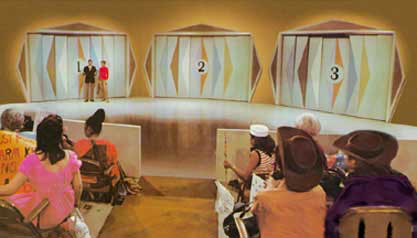
\includegraphics[scale=.5]{Doors}\end{center}
\begin{itemize}
\item Parade received 10,000 angry letters from readers who thought
vos Savant wrong
\item 1000 letters from readers with PhDs
\item Famous mathematician
Paul Erd\"os unconvinced until shown computer simulation
\end{itemize}
\end{frame}

\begin{frame}
\begin{itemize}
\item Example of letter from angry reader:
\item\begin{quotation}
``You blew it, and you blew it big! Since you seem to have difficulty
grasping the basic principle at work here, I'll explain. After the
host reveals a goat, you now have a one-in-two chance of being
correct. Whether you change your selection or not, the odds are the
same. There is enough mathematical illiteracy in this country, and
we don't need the world's highest IQ propagating more. Shame!''
\end{quotation}
\item[] --Scott Smith, Ph.D. University of Florida
\end{itemize}
\begin{remark}
\begin{itemize}
\item Also in 1990 HTTP introduced (i.e. the WWW)
\item Smith couldn't have known in 1990 his comments
would be preserved for all time on web
\item Thus ``flaming'' someone not advisable
\end{itemize}
\end{remark}
\end{frame}

\begin{frame}
\begin{itemize}
\item Tree diagram for Monty Hall problem:
\item \alert{$C$} denotes car
\item \alert{$G_1,G_2$} denote goats
\end{itemize}
\[\begin{xy}<1cm,0cm>:
(-6,-1)*{\text{You choose:}};
(-6,-2)*{\text{Host shows you:}};
(0,0)="0";
(-3,-1)="-31";
(0,-1)="01";
(3,-1)="31";
"0";"-31"*+!D{C}**\dir{-};
"0";"01"*+!D{G_1}**\dir{-};
"0";"31"*+!D{G_2}**\dir{-};
"-31";(-4,-2)*{G_1}**\dir{-};
"-31";(-2,-2)*{G_2}**\dir{-};
"01";(0,-2)*{G_2}**\dir{-};
"31";(3,-2)*{G_1}**\dir{-};
\end{xy}\]
\end{frame}

\begin{frame}
\[\begin{xy}<1cm,0cm>:
(-6,-1)*{\text{You choose:}};
(-6,-2)*{\text{Host shows you:}};
(-6,-5)*{\text{Probability:}};
(0,0)="0";
(-3,-1)="-31";
(0,-1)="01";
(3,-1)="31";
"0";"-31"*+!D{C}**\dir{-}?*+!D{\frac{1}{3}};
"0";"01"*+!D{G_1}**\dir{-}?*+!DL{\frac{1}{3}};
"0";"31"*+!D{G_2}**\dir{-}?*+!D{\frac{1}{3}};
"-31";(-4,-2)*{G_1}**\dir{-}?*+!R{\frac{1}{2}};
"-31";(-2,-2)*{G_2}**\dir{-}?*+!L{\frac{1}{2}};
"01";(0,-2)*{G_2}**\dir{-};
"31";(3,-2)*{G_1}**\dir{-};
(-4,-5)*{\frac{1}{6}};(-2,-5)*{\frac{1}{6}};
(0,-5)*{\frac{1}{3}};(3,-5)*{\frac{1}{3}};
\end{xy}\]
\end{frame}

\begin{frame}
\[\begin{xy}<1cm,0cm>:
(-6,-1)*{\text{You choose:}};
(-6,-2)*{\text{Host shows you:}};
(-6,-3)*{\text{If you switch:}};
(-6,-5)*{\text{Probability:}};
(0,0)="0";
(-3,-1)="-31";
(0,-1)="01";
(3,-1)="31";
"0";"-31"*+!D{C}**\dir{-}?*+!D{\frac{1}{3}};
"0";"01"*+!D{G_1}**\dir{-}?*+!DL{\frac{1}{3}};
"0";"31"*+!D{G_2}**\dir{-}?*+!D{\frac{1}{3}};
"-31";(-4,-2)*{G_1}**\dir{-}?*+!R{\frac{1}{2}};
"-31";(-2,-2)*{G_2}**\dir{-}?*+!L{\frac{1}{2}};
"01";(0,-2)*{G_2}**\dir{-};
"31";(3,-2)*{G_1}**\dir{-};
(-4,-3)*{L};(-2,-3)*{L};(0,-3)*{W};(3,-3)*{W};
(-4,-5)*{\frac{1}{6}};(-2,-5)*{\frac{1}{6}};
(0,-5)*{\frac{1}{3}};(3,-5)*{\frac{1}{3}};
\end{xy}\]
So $\frac{1}{3}+\frac{1}{3}=\frac{2}{3}$ the
probability of winning if you switch
\end{frame}

\begin{frame}
\[\begin{xy}<1cm,0cm>:
(-6,-1)*{\text{You choose:}};
(-6,-2)*{\text{Host shows you:}};
(-6,-3)*{\text{If you switch:}};
(-6,-4)*{\text{If you stay:}};
(-6,-5)*{\text{Probability:}};
(0,0)="0";
(-3,-1)="-31";
(0,-1)="01";
(3,-1)="31";
"0";"-31"*+!D{C}**\dir{-}?*+!D{\frac{1}{3}};
"0";"01"*+!D{G_1}**\dir{-}?*+!DL{\frac{1}{3}};
"0";"31"*+!D{G_2}**\dir{-}?*+!D{\frac{1}{3}};
"-31";(-4,-2)*{G_1}**\dir{-}?*+!R{\frac{1}{2}};
"-31";(-2,-2)*{G_2}**\dir{-}?*+!L{\frac{1}{2}};
"01";(0,-2)*{G_2}**\dir{-};
"31";(3,-2)*{G_1}**\dir{-};
(-4,-3)*{L};(-2,-3)*{L};(0,-3)*{W};(3,-3)*{W};
(-4,-4)*{W};(-2,-4)*{W};(0,-4)*{L};(3,-4)*{L};
(-4,-5)*{\frac{1}{6}};(-2,-5)*{\frac{1}{6}};
(0,-5)*{\frac{1}{3}};(3,-5)*{\frac{1}{3}};
\end{xy}\]
So $\frac{1}{6}+\frac{1}{6}=\frac{1}{3}$ the
probability of winning if you stay
\end{frame}

\begin{frame}
\begin{itemize}
\item Alternate explanation:
\item You choose door 1
\item $\frac{1}{3}$ the probability that car behind door 1
\item So $\frac{2}{3}$ the probability that car behind
door 2 or 3
\item Subsequent events don't change these facts
\item Host shows you goat behind door 3
\item $\frac{2}{3}$ still the probability that car behind
door 2 or 3
\item \dots but now we know that car \alert{not} behind
door 3
\item So car behind door 2 with probability $\frac{2}{3}$
\item Conclusion: should switch to door 2
\end{itemize}
\end{frame}

\end{document} 
